\section{Implementación}

En esta sección, se detalla la implementación del sistema de generación de terreno procedural en Unity. Se describe en profundidad la estructura de la herramienta, la implementación de los algoritmos y la resolución de problemas encontrados durante el desarrollo.

\subsection{Implementación de la Arquitectura}

En esta subsección, se aborda la implementación detallada de la estructura de la herramienta en Unity. Se describen los scripts y la organización de los componentes que conforman la arquitectura del sistema.

\subsubsection{Scripts y Componentes Clave}

Se presentan y explican los scripts y componentes clave que forman parte de la arquitectura del sistema, incluyendo su función y relación con otros elementos.

\begin{enumerate}
    \item \textbf{EndlessTerrain}:
    La clase \texttt{EndlessTerrain} es la clase de unity que implementa la generación de chunks de terreno infinita, la cual se ha traducido en código de la siguiente forma.

    Consta de los siguientes \texttt{atributos:}

    \begin{itemize}
        \item \texttt{Scale}: Escala utilizada para ajustar la posición del terreno.
        \item \texttt{ViewerMoveThresholdForChunkUpdate}: Umbral de movimiento del espectador para actualizar chunks.
        \item \texttt{SqrViewerMoveThresholdForChunkUpdate}: Umbral de movimiento al cuadrado.
        \item \texttt{detailLevels}: Niveles de detalle (LOD) del terreno.
        \item \texttt{ maxViewDst}: Máxima distancia de visualización.
        \item \texttt{viewer}: Transform del espectador.
        \item \texttt{ mapMaterial}: Material del mapa.
        \item \texttt{viewerPosition}: Posición del espectador.
        \item \texttt{\_viewerPositionOld}: Posición anterior del espectador.
        \item \texttt{\_mapGenerator}: Instancia del generador de mapas.
        \item \texttt{\_chunkSize}: Tamaño de los chunks del mapa.
        \item \texttt{\_chunksVisibleInViewDst}: Cantidad de chunks visibles en la distancia.
        \item \texttt{\_terrainChunkDictionary}: Diccionario que almacena los chunks de terreno.
        \item \texttt{\_terrainChunksVisibleLastUpdate}: Lista de chunks visibles en la última actualización.
    \end{itemize}

    \texttt{Métodos Principales}

    \begin{itemize}
        \item \texttt{void Start()}: Inicializa la clase.
        \item \texttt{void Update()}: Actualiza la posición del espectador y gestiona la actualización de chunks.
        \item \texttt{void UpdateVisibleChunks()}: Actualiza la visibilidad de los chunks de terreno en función de la posición del espectador.
    \end{itemize}

    \texttt{Funcionalidad:}

    En la subseccion \ref{subsec:generacion-infinita} se profundiza en el método en que se genera el terrneo infinito.\\
    \\

    \item \textbf{TerrainChunk}:

    La clase \texttt{TerrainChunk} es la encargada de representar y gestionar un chunk de terreno individual en Unity. A continuación, se detallan sus atributos y métodos clave:

    \texttt{Atributos:}

    \begin{itemize}
        \item \texttt{\_meshObject}: Objeto de juego que representa el chunk de terreno.
        \item \texttt{\_position}: Posición del chunk en coordenadas locales.
        \item \texttt{\_bounds}: Área delimitada que abarca el chunk.
        \item \texttt{\_meshRenderer}: Componente para la representación visual del terreno.
        \item \texttt{\_meshFilter}: Componente para gestionar la malla del terreno.
        \item \texttt{\_meshCollider}: Componente para las colisiones del terreno.
        \item \texttt{\_detailLevels}: Niveles de detalle (LOD) disponibles.
        \item \texttt{\_lodMeshes}: Array de objetos LODMesh para cada nivel de detalle.
        \item \texttt{\_mapData}: Datos del mapa asociados a este chunk.
        \item \texttt{\_mapDataReceived}: Indica si los datos del mapa han sido recibidos.
        \item \texttt{\_previousLODIndex}: Índice del nivel de detalle (LOD) previamente utilizado.
    \end{itemize}

    \texttt{Métodos Principales:}

    \begin{itemize}
        \item \texttt{TerrainChunk(Vector2 coord,  size, LODInfo[] detailLevels, Transform parent, Material material)}: Constructor de la clase que inicializa un chunk de terreno.
        \item \texttt{void OnMapDataReceived(MapData mapData)}: Callback llamado cuando se reciben los datos del mapa.
        \item \texttt{void UpdateTerrainChunk()}: Actualiza la visibilidad y el nivel de detalle del chunk.
        \item \texttt{void SetVisible(bool visible)}: Establece la visibilidad del chunk.
        \item \texttt{bool IsVisible()}: Verifica si el chunk es visible.
    \end{itemize}

    \texttt{Funcionalidad:}

    La clase \texttt{TerrainChunk} es responsable de representar un chunk específico del terreno. Cuando se crea un objeto de esta clase, se inicializa con sus atributos y se solicitan los datos del mapa asociados a ese chunk. Luego, durante la actualización, se verifica si el chunk debe ser visible en función de su distancia al espectador y se ajusta su nivel de detalle (LOD) en consecuencia. Finalmente, se gestiona la visibilidad del chunk y su representación visual.\\
    \\

    \item \textbf{LODMesh}:

    La clase \texttt{LODMesh} se encarga de gestionar las mallas de diferentes niveles de detalle (LOD) utilizadas en la representación del terreno. Aquí se detallan sus atributos y métodos clave:

    \texttt{Atributos:}

    \begin{itemize}
        \item \texttt{mesh}: Representa la malla del terreno para un nivel de detalle (LOD) específico.
        \item \texttt{hasRequestedMesh}: Indica si se ha solicitado la generación de la malla.
        \item \texttt{hasMesh}: Indica si la malla está disponible.
        \item \texttt{\_lod}: Nivel de detalle (LOD) asociado a esta malla.
        \item \texttt{\_updateCallback}: Callback que se llama cuando se recibe la malla.
    \end{itemize}

    \texttt{Métodos Principales:}

    \begin{itemize}
        \item \texttt{void OnMeshDataReceived(MeshData meshData)}: Callback llamado cuando se reciben los datos de la malla.
        \item \texttt{void RequestMesh(MapData mapData)}: Solicita la generación de la malla asociada a este LOD.
    \end{itemize}

    \texttt{Funcionalidad:}

    La clase \texttt{LODMesh} gestiona las mallas correspondientes a diferentes niveles de detalle del terreno. Cuando se crea un objeto de esta clase, se establece el nivel de detalle (LOD) y un callback que se ejecutará cuando la malla esté disponible. La función \texttt{RequestMesh} inicia la solicitud de generación de la malla.\\
    \\

    \item \textbf{LODInfo}:

    La estructura \texttt{LODInfo} almacena información sobre los niveles de detalle (LOD) utilizados para optimizar la representación del terreno. A continuación, se detallan sus atributos:

    \texttt{Atributos:}

    \begin{itemize}
        \item \texttt{lod}: Representa el nivel de detalle (LOD).
        \item \texttt{visibleDstThreshold}: Define la distancia a la que se activa este nivel de detalle.
    \end{itemize}

    \texttt{Funcionalidad:}

    La estructura \texttt{LODInfo} se utiliza para configurar los niveles de detalle (LOD) y establecer los umbrales de distancia a los cuales se activa cada nivel. Esto permite optimizar la representación del terreno en función de la proximidad al espectador.\\
    \\
 
    \item \textbf{MapGenerator}:

    La clase \texttt{MapGenerator} es responsable de generar y gestionar los datos del mapa, así como de generar mallas de terreno en Unity. A continuación, se describen sus atributos y métodos clave:

    \texttt{Atributos:}

    \begin{itemize}
        \item \texttt{ MapChunkSize}: Tamaño de los chunks del mapa.
        \item \texttt{configSettings}: Configuración del generador de mapas.
        \item \texttt{colorGradient}: Gradiente de colores utilizado para asignar colores al terreno.
        \item \texttt{\_batchSize}: Tamaño del lote para las operaciones en paralelo.
    \end{itemize}

    \texttt{Métodos Principales:}

    \begin{itemize}
        \item \texttt{void DrawMapInEditor()}: Dibuja el mapa en el editor de Unity.
        \item \texttt{void RequestMapData(Vector2 centre, Action<MapData> callback)}: Solicita datos del mapa en una ubicación específica y llama a un callback cuando los datos están listos.
        \item \texttt{void RequestMeshData(MapData mapData,  lod, Action<MeshData> callback)}: Solicita datos de malla del terreno y llama a un callback cuando la malla está lista.
    \end{itemize}

    \texttt{Funcionalidad:}

    La clase \texttt{MapGenerator} se encarga de generar datos del mapa y mallas de terreno en función de la configuración proporcionada. Puede generar mapas de ruido, mapas de colores y mallas de terreno. Los métodos \texttt{RequestMapData} y \texttt{RequestMeshData} permiten solicitar estos datos y mallas de manera asincrónica.

    Además, la clase realiza la erosión del terreno si la configuración así lo indica, aplicando un número específico de ciclos de erosión al mapa de alturas.

    También se encarga de la generación de mallas de terreno a diferentes niveles de detalle (LOD) utilizando el sistema de jobs de Unity para un rendimiento óptimo.\\
    \\

    \item \textbf{MapData}:

    La estructura \texttt{MapData} almacena los datos generados del mapa, incluido el mapa de alturas y el mapa de colores. A continuación, se describen sus atributos:

    \texttt{Atributos:}

    \begin{itemize}
        \item \texttt{[] heightMap}: Mapa de alturas del terreno.
        \item \texttt{Color[] colourMap}: Mapa de colores del terreno.
    \end{itemize}

    \texttt{Funcionalidad:}

    La estructura \texttt{MapData} proporciona una forma de encapsular y transportar los datos generados del mapa entre diferentes partes del programa. Almacena tanto el mapa de alturas como el mapa de colores para su uso en la representación del terreno.\\
    \\

    \item \textbf{MapDataGeneratorJob}:

    La estructura \texttt{MapDataGeneratorJob} representa un trabajo en paralelo utilizado para generar datos del mapa, incluyendo el mapa de alturas y el mapa de colores del terreno. A continuación, se describen sus atributos y métodos clave:

    \texttt{Atributos:}

    \begin{itemize}
        \item \texttt{\_heightMap}: Un array nativo que almacena el mapa de alturas del terreno.
        \item \texttt{\_colMap}: Un array nativo que almacena el mapa de colores del terreno.
        \item \texttt{\_heightMapSettings}: Configuración de generación del mapa de alturas, que incluye detalles como octavas, frecuencia y amplitud.
        \item \texttt{\_mapChunkSize}: El tamaño del chunk del mapa.
        \item \texttt{\_centre}: El centro del mapa en coordenadas 2D.
        \item \texttt{\_colorGradient}: Un array nativo que almacena una paleta de colores utilizada para mapear alturas a colores.
    \end{itemize}

    \texttt{Métodos Principales:}

    \begin{itemize}
        \item \texttt{MapDataGeneratorJob(HeightMapSettings heightMapSettings, \\int mapChunkSize, float2 centre, NativeArray<Color> colorGradient)}: Constructor de la estructura \texttt{MapDataGeneratorJob} que recibe la configuración del mapa de alturas, el tamaño del chunk del mapa, el centro del mapa y la paleta de colores.

        \item \texttt{Execute(int threadIndex)}: Método que se ejecuta en paralelo para generar datos del mapa en una posición específica. Calcula la altura en esa posición y asigna un color correspondiente basado en la paleta de colores.

        \item \texttt{ReturnMapData()}: Método que devuelve los datos generados del mapa, incluyendo el mapa de alturas y el mapa de colores, en forma de una estructura \texttt{MapData}.

        \item \texttt{Dispose()}: Método que se encarga de liberar los recursos utilizados por los arrays nativos \texttt{\_colMap} y \texttt{\_heightMap} una vez que se han generado los datos del mapa.

    \end{itemize}

    La estructura \texttt{MapDataGeneratorJob} es esencial en el proceso de generación de terreno, ya que calcula y asigna alturas y colores a cada punto del mapa en paralelo, lo que permite una generación eficiente del terreno.\\
    \\

    \item \textbf{Noise}:

    La clase `Noise` es una utilidad que proporciona métodos para generar mapas de ruido, que se utilizan en la generación de terrenos. Esta clase contiene una enumeración `Type` que define los tipos de ruido disponibles, como Perlin, Simplex y Voronoi.

    \texttt{Métodos Principales:}

    \begin{itemize}
        \item \texttt{GenerateNoiseMap(int mapSize, HeightMapSettings parameters, float2 centre)}: Este método genera un mapa de ruido basado en parámetros dados, como el tamaño del mapa, la configuración de mapas de alturas y el centro del mapa. Utiliza el ruido Perlin para calcular alturas y devuelve un array de floats que representa el mapa de ruido generado.

        \item \texttt{GenerateNoiseValue(float2 position, HeightMapSettings parameters)}: Este método genera un valor de ruido en una posición dada utilizando los parámetros de configuración y la posición proporcionada. Puede utilizar diferentes tipos de ruido según los parámetros. Devuelve un valor de ruido float en función de la posición.

        \item \texttt{SampleNoiseValue(float2 sample, Type type)}: Este método toma una muestra de ruido en una posición dada utilizando el tipo de ruido especificado. Puede ser Perlin, Simplex o Voronoi. Devuelve un valor de ruido float en función del tipo de ruido y la posición de la muestra.

    \end{itemize}

    La clase `Noise` es esencial en la generación de terrenos, ya que proporciona las herramientas para generar mapas de ruido que se utilizan para determinar las alturas y características del terreno, lo que contribuye a la variedad y realismo del entorno generado.\\
    \\

    \item \textbf{MeshGenerator}:

    La clase \texttt{MeshGenerator} es una clase estática que se encarga de generar las mallas de terreno para el sistema de generación de terreno en Unity. A continuación, se describen sus atributos y métodos clave:

    \texttt{Métodos Principales:}

    \begin{itemize}
        \item \texttt{ MeshData GenerateTerrainMesh([] heightMap, MeshSettings parameters,  size,  levelOfDetail)}: Genera una malla de terreno a partir de un mapa de alturas y una configuración dada. Esta función calcula los vértices, triángulos y coordenadas UV de la malla en función de los parámetros proporcionados.

        \texttt{Atributos:}

        \begin{itemize}
            \item \texttt{topLeftX}: Coordenada X del vértice superior izquierdo del terreno.
            \item \texttt{topLeftZ}: Coordenada Z del vértice superior izquierdo del terreno.
            \item \texttt{meshSimplificationIncrement}: Incremento de simplificación de malla para LOD.
            \item \texttt{verticesPerLine}: Número de vértices por línea en la malla.
            \item \texttt{MeshData meshData}: Objeto que almacena los datos de la malla, incluyendo vértices, triángulos y coordenadas UV.
            \item \texttt{vertexIndex}: Índice actual del vértice.
        \end{itemize}

        Esta función recorre el mapa de alturas y genera los vértices de la malla en función de la altura de cada punto en el mapa. También calcula los triángulos que forman la malla y las coordenadas UV para mapear texturas.
    \end{itemize}

    La clase \texttt{MeshGenerator} es esencial para la generación de mallas de terreno y su adaptación a diferentes niveles de detalle (LOD) en el sistema de generación de terreno en Unity.\\
    \\

    \item \textbf{MeshData}: Esta estructura almacena los datos de una malla de terreno, incluyendo los vértices, triángulos, coordenadas UV y un índice de triángulo actual.

    \texttt{Atributos:}

    \begin{itemize}
        \item \texttt{vertices}: Array de vectores que representan los vértices de la malla.
        \item \texttt{triangles}: Array de enteros que define los triángulos de la malla.
        \item \texttt{uvs}: Array de vectores 2D que almacena las coordenadas UV de la malla.
        \item \texttt{triangleIndex}: Índice actual de triángulo.
    \end{itemize}

    \texttt{Funcionalidad:}

    La estructura \texttt{MeshData} proporciona una forma de almacenar y transportar los datos de una malla de terreno. Además, incluye un método para añadir triángulos y otro para crear una malla Unity a partir de los datos almacenados.\\
    \\

    \item \textbf{MeshDataGeneratorJob}:

    La estructura \texttt{MeshDataGeneratorJob} representa un trabajo en paralelo utilizado para generar datos de malla para el terreno. Su objetivo principal es calcular las coordenadas de vértices, coordenadas UV y triángulos de la malla del terreno en función de un mapa de alturas. A continuación, se describen sus atributos y métodos clave:

    \texttt{Atributos:}

    \begin{itemize}
        \item \texttt{\_size}: El tamaño de la malla.
        \item \texttt{\_meshSimpplificationIncrement}: El incremento de simplificación de la malla.
        \item \texttt{\_meshSettings}: Configuración de la malla, que incluye detalles como la altura del agua.
        \item \texttt{\_heightMap}: Un array nativo que almacena el mapa de alturas del terreno.
        \item \texttt{\_vertices}: Un array nativo que almacena las coordenadas de los vértices de la malla.
        \item \texttt{\_uvs}: Un array nativo que almacena las coordenadas UV de la malla.
        \item \texttt{\_triangles}: Un array nativo que almacena la información de los triángulos de la malla.
    \end{itemize}

    \texttt{Métodos Principales:}

    \begin{itemize}
        \item \texttt{MeshDataGeneratorJob(int size, int meshSimplificationIncrement, \\MeshSettings meshSettings, NativeArray<float> heightMap, NativeArray<Vector3> \\vertices, NativeArray<Vector2> uvs, NativeArray<int> triangles)}: Constructor de la estructura \texttt{MeshDataGeneratorJob} que recibe el tamaño de la malla, el incremento de simplificación de la malla, la configuración de la malla, el mapa de alturas, y los arrays nativos para almacenar los datos de la malla.

        \item \texttt{Execute(int index)}: Método que se ejecuta en paralelo para calcular las coordenadas de vértices, coordenadas UV y triángulos de la malla en función de la información del mapa de alturas. Cada hilo de trabajo calcula estos datos para una posición específica en la malla.

    \end{itemize}

    La estructura \texttt{MeshDataGeneratorJob} es esencial en el proceso de generación de la malla del terreno, ya que permite calcular eficientemente las coordenadas de vértices y triángulos, lo que resulta en un terreno visualmente atractivo y detallado.\\
    \\

    \item \textbf{Erosion}:

    La clase \texttt{Erosion} es una clase estática que implementa el proceso de erosión térmica en el contexto del sistema de generación de terreno en Unity. A continuación, se describen sus atributos y métodos clave:

    \texttt{Métodos Principales:}

    \begin{itemize}
        \item \texttt{public static float ThermalErosionValue(int x, int y, int mapChunkSize, ErosionSettings erosionSettings, NativeArray<float> heightMap, float iterFraction)}: Este método calcula el valor erosionado de una posición dada en el mapa de alturas utilizando el proceso de erosión térmica.

        \texttt{Parámetros:}

        \begin{itemize}
            \item \texttt{x, y}: Coordenadas de la posición en el mapa de alturas.
            \item \texttt{mapChunkSize}: Tamaño del chunk del mapa.
            \item \texttt{erosionSettings}: Configuración de erosión que incluye valores como el tamaño del borde y el ángulo de talud.
            \item \texttt{heightMap}: Array nativo que almacena el mapa de alturas.
            \item \texttt{iterFraction}: Fracción de iteración actual (para controlar la erosión en cada iteración).
        \end{itemize}

        Este método calcula el efecto de la erosión térmica en la altura del terreno en una posición específica. Compara la altura actual con la altura de los vecinos y ajusta la altura según el ángulo de talud y la configuración de erosión.

        \item \texttt{private static bool InsideBorder(int x, int y, int borderSize, int mapChunkSize)}: Este método verifica si una posición dada está dentro del área del borde definida por el tamaño del borde.

        \texttt{Parámetros:}

        \begin{itemize}
            \item \texttt{x, y}: Coordenadas de la posición en el mapa de alturas.
            \item \texttt{borderSize}: Tamaño del borde.
            \item \texttt{mapChunkSize}: Tamaño del chunk del mapa.
        \end{itemize}

        Este método se utiliza para determinar si una posición dada está dentro del área del borde, lo que afecta a la aplicación de la erosión térmica en esa posición.

    \end{itemize}

    La clase \texttt{Erosion} desempeña un papel importante en el proceso de generación de terreno, específicamente en la simulación de la erosión térmica que afecta a la topografía del terreno generado.\\
    \\

    \item \textbf{ErosionJob}:

    La estructura \texttt{ErosionJob} representa un trabajo en paralelo que se encarga de aplicar la erosión térmica al mapa de alturas de un terreno. A continuación, se describen sus atributos y métodos clave:

    \texttt{Atributos:}

    \begin{itemize}
        \item \texttt{\_heightMap}: Un array nativo de solo lectura que almacena el mapa de alturas original.
        \item \texttt{\_erodedHeightMap}: Un array nativo que almacena el resultado de la erosión térmica.
        \item \texttt{\_mapChunkSize}: El tamaño del chunk del mapa.
        \item \texttt{\_erosionSettings}: Configuración de erosión que incluye valores como el tamaño del borde y el ángulo de talud.
        \item \texttt{\_iterFraction}: Fracción de iteración actual (para controlar la erosión en cada iteración).
    \end{itemize}

    \texttt{Métodos Principales:}

    \begin{itemize}
        \item \texttt{public ErosionJob(NativeArray<float> heightMap, ErosionSettings \\erosionSettings, int mapChunkSize, float iterFraction)}: Constructor de la estructura \texttt{ErosionJob} que recibe el mapa de alturas original, la configuración de erosión, el tamaño del chunk del mapa y la fracción de iteración actual.

        \texttt{Parámetros:}

        \begin{itemize}
            \item \texttt{heightMap}: Un array nativo que almacena el mapa de alturas original.
            \item \texttt{erosionSettings}: Configuración de erosión que incluye valores como el tamaño del borde y el ángulo de talud.
            \item \texttt{mapChunkSize}: Tamaño del chunk del mapa.
            \item \texttt{iterFraction}: Fracción de iteración actual (para controlar la erosión en cada iteración).
        \end{itemize}

        Este constructor inicializa los atributos de la estructura y crea un nuevo array nativo para almacenar el mapa de alturas erosionado.

        \item \texttt{public void Execute(int threadIndex)}: Método que se ejecuta en paralelo para calcular y aplicar la erosión térmica en una posición específica del mapa de alturas.

        \texttt{Parámetros:}

        \begin{itemize}
            \item \texttt{int threadIndex}: Índice del hilo de ejecución que indica la posición en el mapa de alturas.
        \end{itemize}

        Este método utiliza la función \texttt{Erosion.ThermalErosionValue()} para calcular la erosión en una posición dada y almacena el valor erosionado en el array nativo \texttt{\_erodedHeightMap}.

        \item \texttt{public NativeArray<float> GetErodedHeightMap()}: Método que devuelve el array nativo que contiene el mapa de alturas erosionado.

        \item \texttt{public void Dispose()}: Método que se encarga de liberar los recursos utilizados por el array nativo \texttt{\_erodedHeightMap} una vez que la erosión ha sido aplicada.

    \end{itemize}

    La estructura \texttt{ErosionJob} es fundamental en el proceso de simulación de erosión térmica en el terreno, ya que realiza cálculos paralelos para actualizar el mapa de alturas con los efectos de la erosión.\\
    \\
    \item \textbf{ConfigSettings}:

    La estructura `ConfigSettings` contiene configuraciones generales para la generación de terrenos en Unity. Estas configuraciones se utilizan para controlar aspectos como la vista previa en el editor, las configuraciones del mapa de alturas, la erosión del terreno y las opciones de malla.

    \texttt{Componentes Principales:}

    \begin{itemize}
        \item \texttt{editorPreviewSettings}: Un componente que almacena configuraciones relacionadas con la vista previa en el editor, como el modo de dibujo y la actualización automática.
        
        \item \texttt{heightMapSettings}: Un componente que almacena configuraciones relacionadas con el mapa de alturas, como el tipo de ruido, la escala del ruido y la semilla de generación.
        
        \item \texttt{erosionSettings}: Un componente que almacena configuraciones relacionadas con la erosión del terreno, como la activación de la erosión, la cantidad de ciclos y otros parámetros relacionados con el borde y el ángulo de talud.
        
        \item \texttt{meshSettings}: Un componente que almacena configuraciones relacionadas con la malla de terreno, como el multiplicador de altura de la malla, el nivel del agua y el nivel de detalle de la vista previa en el editor.
    \end{itemize}

    La estructura `ConfigSettings` es esencial para personalizar y controlar cómo se genera y se visualiza el terreno en Unity. Cada componente almacena configuraciones específicas que afectan diferentes aspectos de la generación y visualización del terreno.
\end{enumerate}

\subsection{Implementación de los Algoritmos}

En esta subsección, se profundiza en la implementación de los algoritmos de generación procedimental de terrenos en Unity. Se incluye el código utilizado y se explican las decisiones específicas de implementación.

\subsubsection{Generación Infinita de Chunks de Terreno}

\textbf{Inicio de la generación:}\label{subsec:generacion-infinita}

\begin{itemize}
    \item \textbf{Distancia de Visibilidad}: Se calcula la distancia a la que los chunks serán visibles para el jugador.
    \item \textbf{Tamaño del Chunk}: Se determina el tamaño de cada chunk que se generará.
    \item \textbf{Número de Chunks Visibles}: Se calcula el número de chunks que serán visibles en función de la distancia de visibilidad y el tamaño del chunk.
    \item \textbf{Actualización de chunks visibles}: Se generan los primeros chunks visibles
\end{itemize}
\begin{figure}[h]
    \centering
    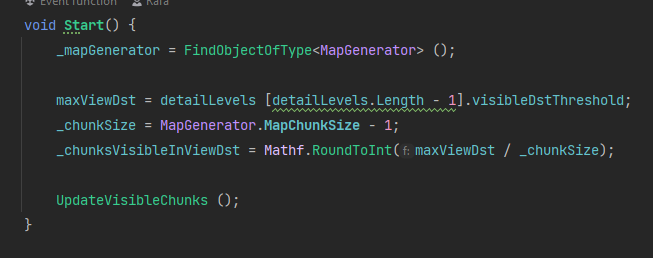
\includegraphics[width=1\textwidth]{img/codes/EndlessTerrain-start.png}
    \caption{Inicialización de parámetros para generación de terreno infinito.}
\end{figure}

\textbf{Actualización de chunks visibles:}

La Actualización de chunks visibles se realiza en la función \texttt{UpdateVisibleChunks} y es donde se gestiona la visibilidad de los chunks de terreno en función de la posición del jugador y se actualizan los chunks que deben estar visibles en la escena.

Para ello esta función realiza los siguientes pasos:

\begin{enumerate}
    \item Recorre la lista \texttt{\_terrainChunksVisibleLastUpdate}, que es una lista de chunks de terreno que estaban visibles en la actualización anterior. Dentro del bucle, se llama al método \texttt{SetVisible(false)} en cada chunk para ocultarlos.
    \item Después de ocultar todos los chunks visibles en la actualización anterior, se borra la lista \texttt{\_terrainChunksVisibleLastUpdate}, preparándola para su uso en la próxima actualización.
    \item Se calculan las coordenadas del chunk actual en el que se encuentra el jugador. Esto se hace dividiendo las coordenadas X e Y de la posición del jugador (\texttt{viewerPosition}) por el tamaño de un chunk (\texttt{\_chunkSize}) y redondeando los resultados a números enteros.
    \item Se inician dos bucles anidados, uno para \texttt{yOffset} (variando desde \\\texttt{-\_chunksVisibleInViewDst} hasta \texttt{\_chunksVisibleInViewDst}) y otro para \texttt{xOffset} (también variando desde \texttt{-\_chunksVisibleInViewDst} hasta \texttt{\_chunksVisibleInViewDst}). Esto se hace para recorrer los chunks en un área cuadrada alrededor del jugador, determinada por \texttt{\_chunksVisibleInViewDst}.
    \item Dentro de los bucles anidados, se calcula \texttt{viewedChunkCoord}, que representa las coordenadas del chunk que se está evaluando actualmente en función de la posición actual del jugador y los desplazamientos \texttt{xOffset} e \texttt{yOffset}.
    \item Luego, se verifica si el diccionario \texttt{\_terrainChunkDictionary} contiene una entrada con las coordenadas \texttt{viewedChunkCoord}. Si existe, significa que el chunk ya ha sido creado previamente, por lo que se llama al método \texttt{UpdateTerrainChunk} en ese chunk para actualizar su visualización en función de la distancia al jugador.
    \item Si no existe una entrada en el diccionario para las coordenadas \texttt{viewedChunkCoord}, significa que el chunk aún no se ha creado. En este caso, se crea un nuevo objeto \texttt{TerrainChunk} con las coordenadas \texttt{viewedChunkCoord}, el tamaño del chunk \texttt{\_chunkSize}, niveles de detalle \texttt{detailLevels}, un transform \texttt{transform}, y un material de mapa \texttt{mapMaterial}. Luego, se agrega este nuevo chunk al diccionario \texttt{\_terrainChunkDictionary}.
\end{enumerate}

Aquí se muestra el código de la función:
\begin{figure}[h]
    \centering
    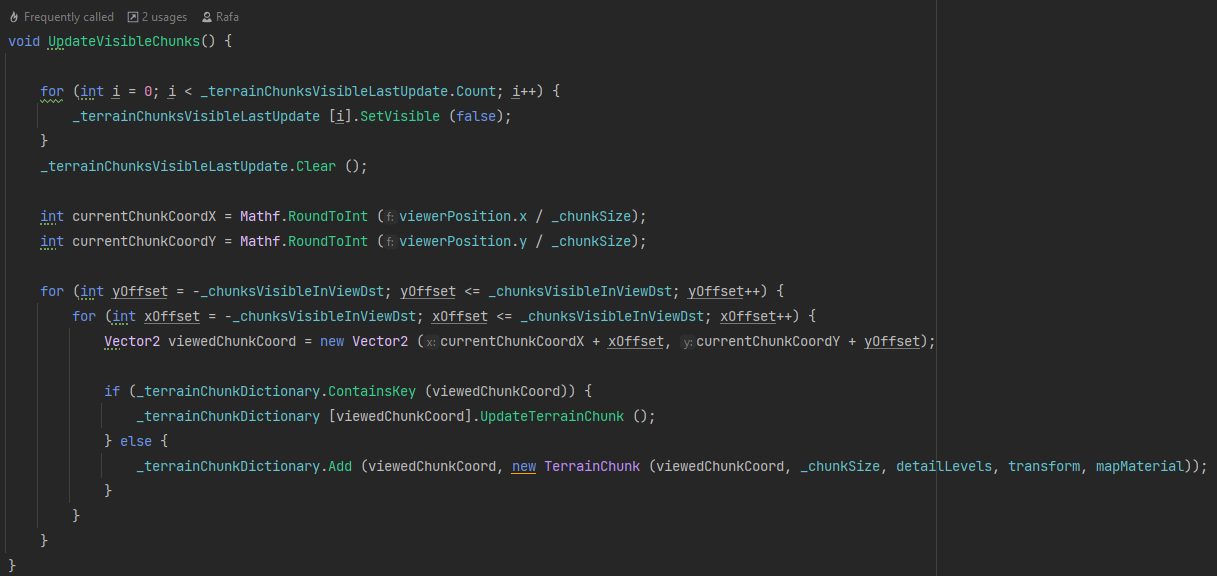
\includegraphics[width=1\textwidth]{img/codes/EndlessTerrain-updateVisibleChunks.png}
    \caption{Carga y descarga de chunks en función de la posición del jugador.}
\end{figure}

\subsubsection{Implementación de Niveles de Detalle (LOD)}

\textbf{Inicialización de parámetros:}

\begin{itemize}
    \item \textbf{Incremento de simplificación de la mesh}: Esta variable controla cuántos vértices se saltan durante la generación de la malla. Si levelOfDetail es 0, no se aplica simplificación, y se establece en 1. Si levelOfDetail es mayor que 0, meshSimplificationIncrement se establece en levelOfDetail * 2, lo que significa que se omiten más vértices en la generación de la malla a medida que aumenta el nivel de detalle.
    \item \textbf{Vértices por línea}:Esta variable determina el número de vértices por línea en la malla. Se calcula dividiendo (size - 1) por meshSimplificationIncrement y sumando 1. Cuanto mayor sea el valor de meshSimplificationIncrement, menor será la cantidad de vértices por línea, lo que resultará en una malla menos detallada.
\end{itemize}
\begin{figure}[h]
    \centering
    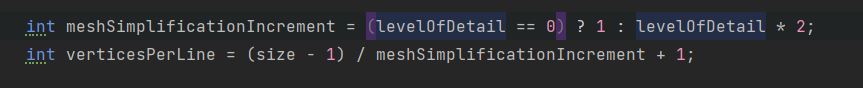
\includegraphics[width=1\textwidth]{img/codes/LOD-parametros.png}
    \caption{Inicialización de variables que implementan LOD.}
\end{figure}

\textbf{Aplicación de las variables de LOD:}

El bucle anidado que recorre el terreno usa meshSimplificationIncrement para determinar cuántos vértices procesar en cada iteración. Cuanto mayor sea meshSimplificationIncrement, menos iteraciones se realizarán en el bucle, lo que significa que se generará menos detalle en la malla. Los vértices omitidos no se incluirán en la malla final.

Triángulos en la malla: Los triángulos que forman la malla se crean en función de la posición de los vértices generados. Si meshSimplificationIncrement es mayor, se omitirán más vértices, lo que resultará en menos triángulos y, por lo tanto, en una malla más simplificada.

Aquí se muestra el código de la función:
\begin{figure}[h]
    \centering
    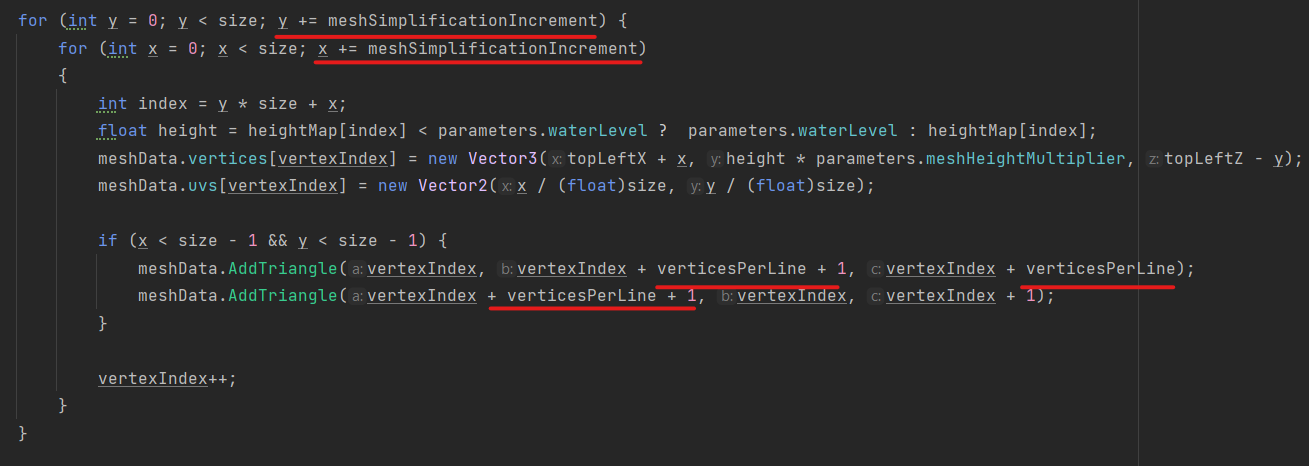
\includegraphics[width=1\textwidth]{img/codes/LOD-bucle.png}
    \caption{Bucle para construir la mesh con LOD.}
\end{figure}

\subsubsection{Generación de Valores de Ruido}

La generación de valores de ruido es un paso fundamental en la creación de terrenos realistas y variados. En este contexto, se utiliza el ruido para determinar las alturas y características del terreno generado. El algoritmo de generación de ruido se implementa en la clase \texttt{Noise} y puede utilizar diferentes tipos de ruido, como Perlin, Simplex o Voronoi, según los parámetros especificados.

\paragraph{Parámetros de Ruido}

Para generar el ruido, se utilizan varios parámetros que influyen en la apariencia del terreno:

\begin{itemize}
    \item \textbf{Tamaño del Mapa (\texttt{mapSize})}: El tamaño del mapa define cuántos puntos se generarán en el mapa de ruido. Cuanto mayor sea este valor, mayor será la resolución del terreno generado.
    
    \item \textbf{Configuración de Altura (\texttt{parameters})}: Esta configuración incluye información como la semilla (\texttt{seed}), la escala del ruido (\texttt{noiseScale}), la persistencia (\texttt{persistance}), la lacunaridad (\texttt{lacunarity}), el número de octavas (\texttt{octaves}) y el desplazamiento (\texttt{offset}). Estos parámetros ajustan cómo se combinarán y generarán los valores de ruido.
    
    \item \textbf{Tipo de Ruido (\texttt{noiseType})}: El algoritmo permite elegir entre diferentes tipos de ruido, como Perlin, Simplex o Voronoi. Cada tipo de ruido tiene un comportamiento único que afecta la apariencia del terreno.
\end{itemize}

\paragraph{Generación de Valores de Ruido}

El algoritmo de generación de ruido comienza con la inicialización de los parámetros, incluidos los desplazamientos aleatorios para cada octava. Luego, se procede a generar los valores de ruido para cada punto en el mapa.

\begin{enumerate}
    \item \textbf{Incialización de Parámetros}: Se generan desplazamientos aleatorios para cada octava, lo que permite variar el patrón de ruido en cada octava y controlar la aparición de detalles a diferentes escalas.
    Aquí se muestra el código:
    \begin{figure}[h]
        \centering
        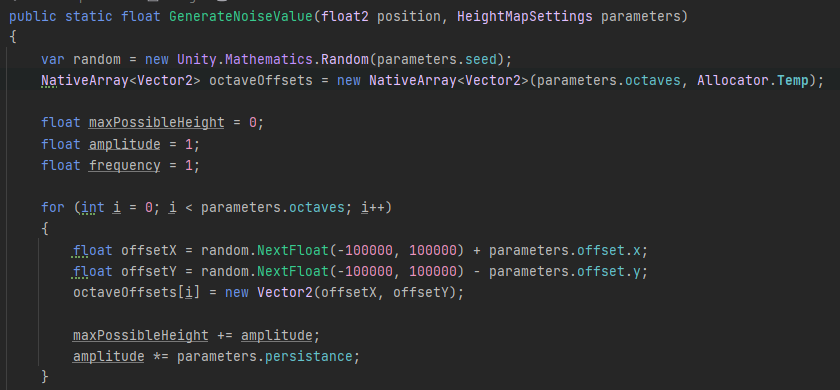
\includegraphics[width=0.9\textwidth]{img/codes/octavas.png}
        \caption{Generación de desplazamientos aleatorios para cada octava.}
    \end{figure}
    
    \item \textbf{Bucle de Generación}: Para cada punto en el mapa de tamaño \texttt{mapSize}, se calcula un valor de ruido. Esto se hace mediante la combinación de múltiples octavas de ruido, cada una escalada y ponderada adecuadamente. La suma de estos valores de ruido se utiliza como altura o característica del terreno en ese punto.
    \begin{figure}[h]
        \centering
        \includegraphics[width=0.9\textwidth]{img/codes/GeneraciónRuido.png}
        \caption{Generación de valores de ruido basado en parámeteros.}
    \end{figure}
    \item \textbf{Nótese cómo en el bucle de generación se multiplican los valores frecuencia y amplitud por la lacunaridad y la Persistencia respectivamente de manera que se aplican estos parámetrod en cada octava}
    \item \textbf{Normalización}: Los valores de ruido generados no están en el rango deseado. Se realiza una normalización para ajustar estos valores al rango [0, 1], que es más adecuado para representar alturas.
    \begin{figure}[h]
        \centering
        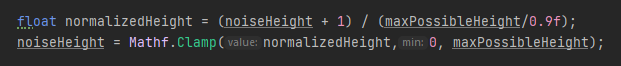
\includegraphics[width=0.9\textwidth]{img/codes/normalizacion.png}
        \caption{Normalización de los valores de ruido generados.}
    \end{figure}
\end{enumerate}

\paragraph{Tipo de Ruido}

El tipo de ruido utilizado afecta significativamente la apariencia del terreno:

\begin{itemize}
    \item \textbf{Perlin}: Este tipo de ruido proporciona un aspecto suave y ondulado al terreno. Es especialmente útil para crear formaciones de terreno natural, como colinas y montañas.
    
    \item \textbf{Simplex}: El ruido Simplex es conocido por su capacidad para generar terrenos más naturales y sin patrones visibles. Puede ser útil para terrenos detallados y variados.
    
    \item \textbf{Voronoi}: El ruido Voronoi se utiliza para crear patrones celulares y características geométricas en el terreno. Puede generar formaciones de terreno únicas y distintivas.
\end{itemize}

\begin{figure}[h]
    \centering
    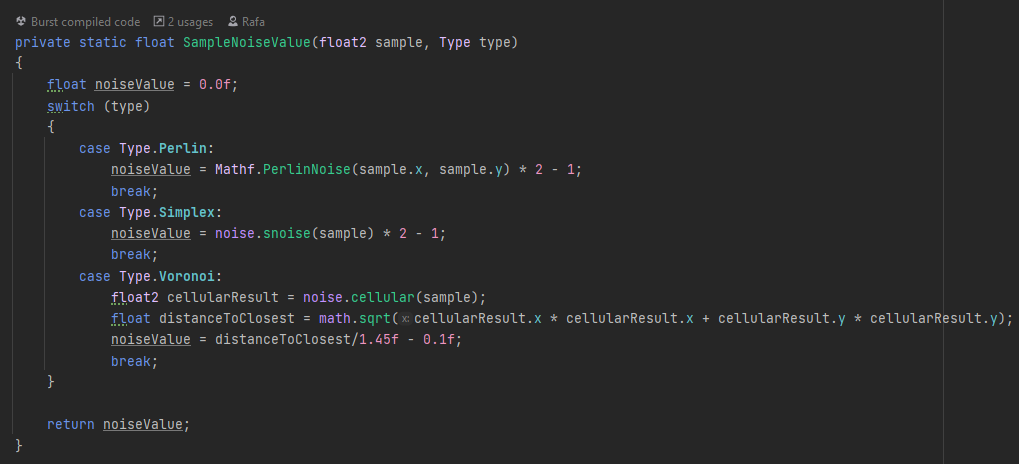
\includegraphics[width=1\textwidth]{img/codes/TiposRuido.png}
    \caption{Función para genrar un valor de ruido u otro en base al tipo seleccionado.}
\end{figure}

\subsubsection{Generación del Mapa de Altura}

\textbf{Llamada al Job desde clase Monobehaviour:}

La generación del mapa de altura se realiza mediante la ejecución de un job de Unity llamado MapDataGeneratorJob. Este job se encarga de calcular las alturas en función de las configuraciones proporcionadas y genera el mapa de altura correspondiente. La ejecución del job se realiza en paralelo, lo que aprovecha el rendimiento de sistemas multi-núcleo.

El Job es llamado desde un método en la clase Monobehaviour que hacede interfaz entre el Job y EndlessTerrain. En la siguiente imagen se observa el código donde se genera el gradiente de color y se hace la llamada al Job:
\begin{figure}[h]
    \centering
    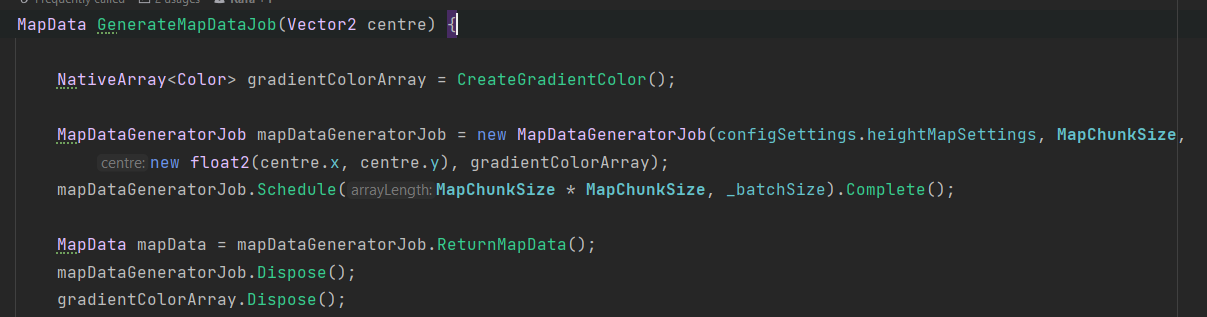
\includegraphics[width=0.9\textwidth]{img/codes/MapGenerator-GenerateMapData.png}
    \caption{Implementación del job MapDataGeneratorJob para la generación del mapa de altura.}
    \end{figure}

\textbf{Job:}

\begin{itemize}
\item \textbf{Cálculo de Alturas}: En cada iteración del job, se calcula la altura del terreno en una posición específica. Esto se logra utilizando funciones de ruido y las configuraciones de altura del terreno.
\item \textbf{Asignación de Colores}: Para cada punto en el mapa de altura, se asigna un color correspondiente utilizando la paleta de colores. Esta asignación se basa en la altura calculada previamente.

Aquí se muestra el código del método execute del MapDataGeneratorJob donde se obtiene la altura y el color para un vértice:
\begin{figure}[h]
    \centering
    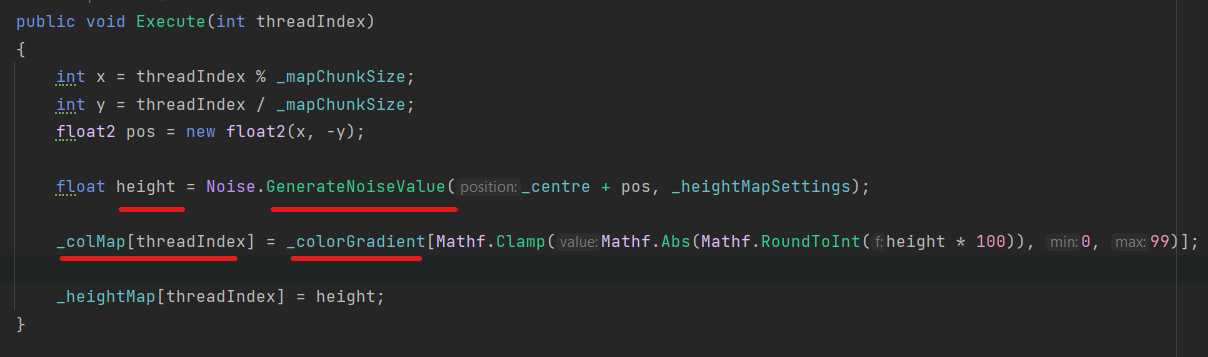
\includegraphics[width=0.9\textwidth]{img/codes/GenracionAlturaYColores.png}
    \caption{Generación de altura y color para un vértice.}
\end{figure}

\item \textbf{MapData Resultante}: El resultado de la generación del mapa de altura se encapsula en una estructura MapData, que contiene tanto el mapa de altura como el mapa de color.
\end{itemize}
\begin{figure}[h]
    \centering
    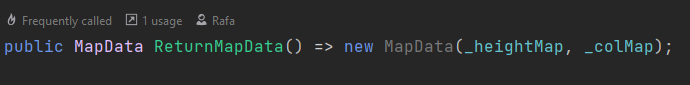
\includegraphics[width=0.9\textwidth]{img/codes/MapDataReturn.png}
    \caption{Generación de la estructura MapData con los datos.}
\end{figure}

Con la finalización de este proceso, se obtiene un mapa de altura que sirve como base para la generación del terreno y contribuye significativamente a su aspecto y forma finales.

Este mapa de altura se utiliza posteriormente en la creación de las mallas del terreno y en otros procesos relacionados con la generación procedural.

\subsubsection{Generación de las Mallas del Terreno}

\textbf{Llamada al Job desde Clase MonoBehaviour:}

La generación de la malla del terreno se lleva a cabo mediante la ejecución de un job de Unity llamado MeshDataGeneratorJob. Este job se encarga de calcular los vértices, triángulos y coordenadas UV de la malla en función de los datos del mapa de altura proporcionados. La ejecución del job se realiza en paralelo, lo que optimiza el rendimiento de la generación de mallas para terrenos de gran escala.

La llamada al job se efectúa desde un método en la clase MonoBehaviour que actúa como intermediario entre el job y el componente EndlessTerrain. En la siguiente imagen se muestra el código donde se crea un job de generación de malla y se ejecuta:

\begin{figure}[h]
\centering
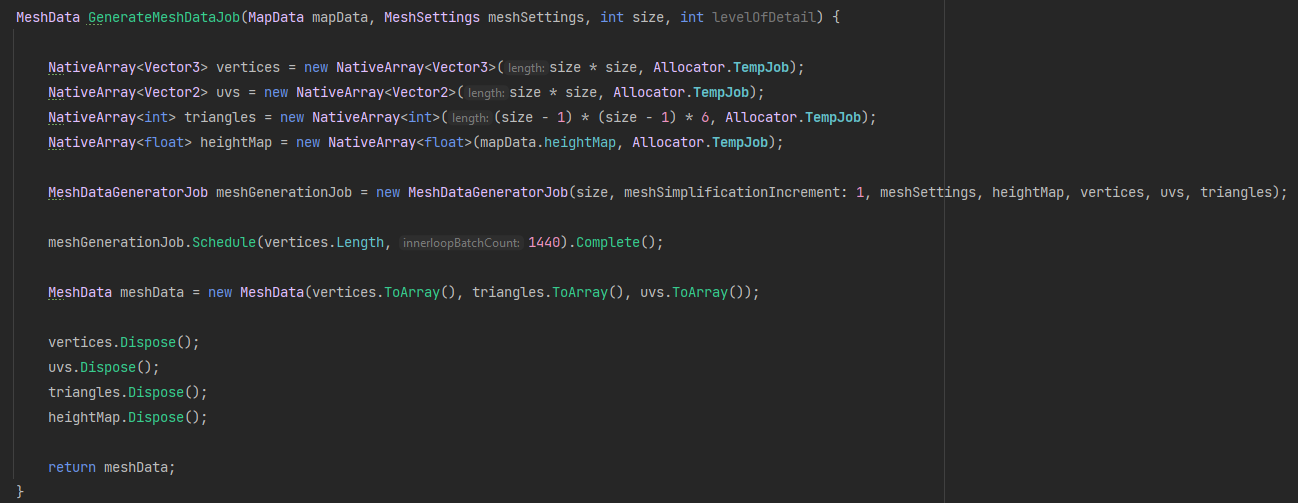
\includegraphics[width=1\textwidth]{img/codes/GenerateMeshData.png}
\caption{Implementación del job MeshDataGeneratorJob para la generación de la malla del terreno.}
\end{figure}

\textbf{Job:}

El job MeshDataGeneratorJob es responsable de generar los datos necesarios para crear la malla del terreno. A continuación, se describen los pasos clave de este proceso:

\begin{itemize}
\item \textbf{Cálculo de Vértices y Coordenadas UV}: En cada iteración del job, se calcula la posición de un vértice en la malla. La altura del vértice se obtiene a partir de los datos del mapa de altura, y las coordenadas UV se asignan en función de la posición en el terreno. Esto permite mapear texturas sobre la malla de manera adecuada. 

\begin{figure}[h]
    \centering
    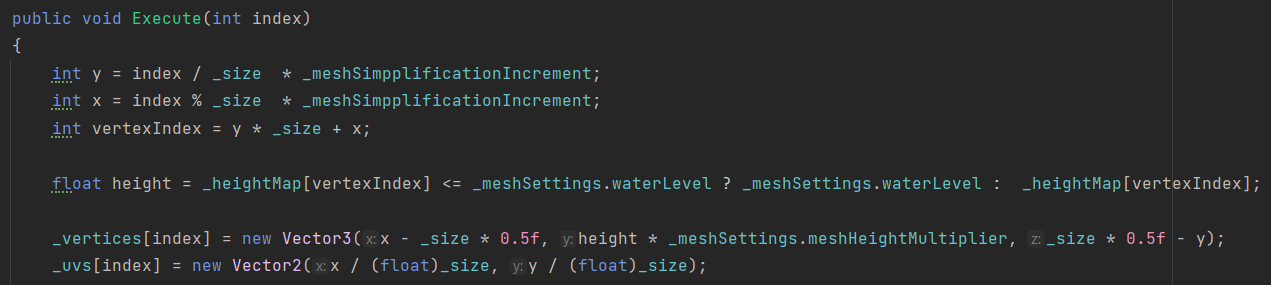
\includegraphics[width=1\textwidth]{img/codes/CalculoVerticesYUVs.png}
    \caption{Cálculo de los vértices y uvs en método Execute del Job.}
\end{figure}

\item \textbf{Creación de Triángulos}: Los triángulos que forman la malla se definen en función de los vértices calculados. Los triángulos determinan la conectividad de la malla y son esenciales para su representación gráfica.
\begin{figure}[h]
    \centering
    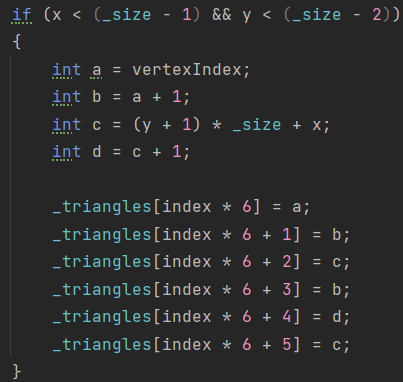
\includegraphics[width=0.5\textwidth]{img/codes/CalculoTriangulos.png}
    \caption{Cálculo de los triángulos en método Execute del Job.}
\end{figure} 
\item \textbf{Resultados en una Estructura}: Los datos generados, incluyendo los vértices, triángulos y coordenadas UV, se encapsulan en una estructura MeshData. Esta estructura almacena todos los elementos necesarios para construir la malla del terreno.
\begin{figure}[h]
    \centering
    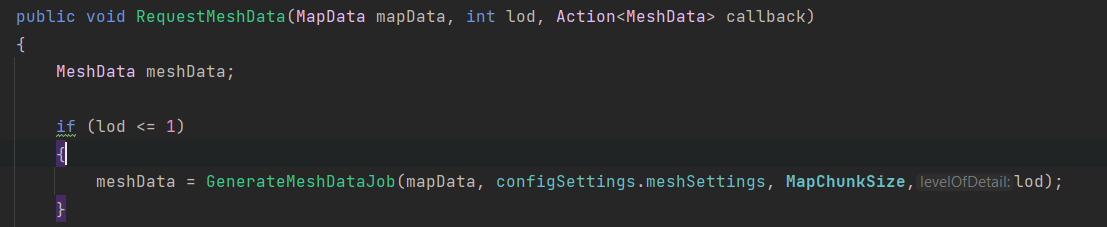
\includegraphics[width=1\textwidth]{img/codes/CreacionMeshData.png}
    \caption{Encapsulación de la información de la mesh en estructura MeshData.}
\end{figure}  
\end{itemize}

Con la finalización de este proceso, se obtiene una malla detallada que representa el terreno procedimental. El uso de jobs en paralelo permite una generación eficiente de la malla, lo que es fundamental para la representación de terrenos complejos y de gran escala en tiempo real.

\subsubsection{Aplicación de Algoritmos de Erosión}

\textbf{Llamada a la Erosión desde Clase MonoBehaviour:}

La aplicación de algoritmos de erosión en el terreno se logra mediante la función ApplyErosion, que utiliza un job de Unity llamado ErosionJob. La erosión es un proceso iterativo que simula la degradación del terreno con el tiempo. La función aplica erosión al mapa de alturas del terreno en múltiples ciclos, donde cada ciclo representa una iteración de erosión. El número de ciclos y otros parámetros de erosión se toman de la configuración.

En el siguiente código, se muestra cómo se llama a la función ApplyErosion y se ejecutan los ciclos de erosión:

\begin{figure}[h]
    \centering
    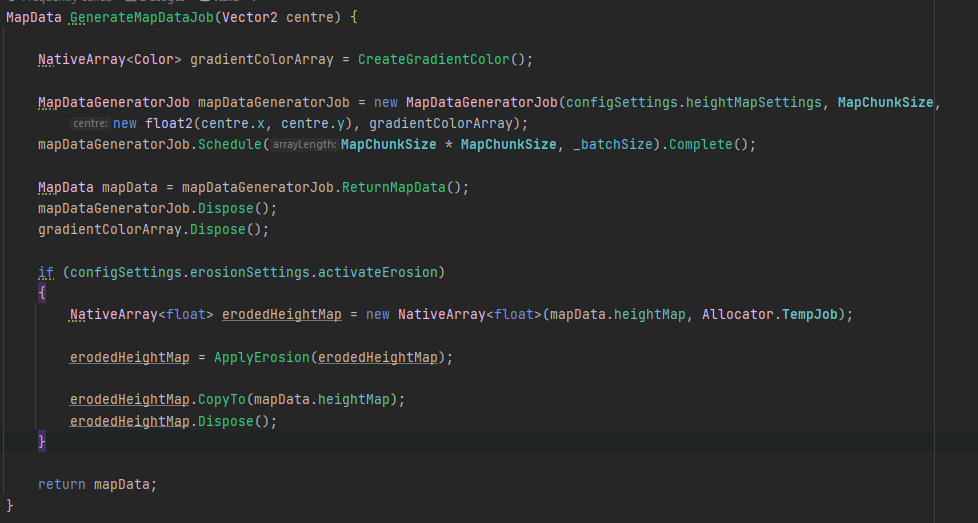
\includegraphics[width=1\textwidth]{img/codes/ApplyErosionCall.png}
    \caption{Llamada a ApplyErosion.}
\end{figure}  

\begin{figure}[h]
    \centering
    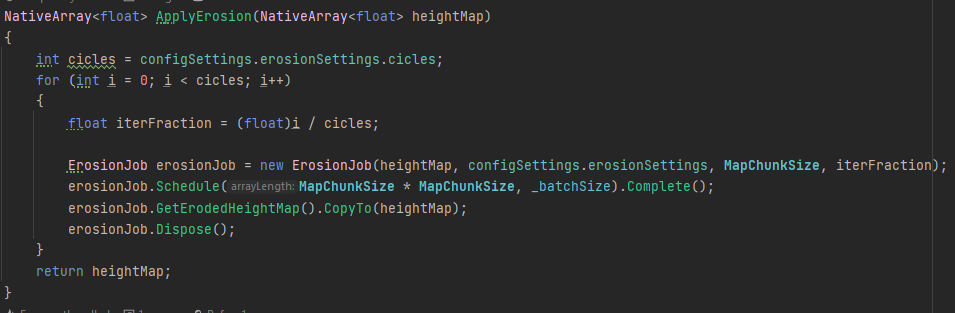
\includegraphics[width=1\textwidth]{img/codes/ApplyErosionFunction.png}
    \caption{Aplicación de la erosión.}
\end{figure} 

\textbf{Job de Erosión (ErosionJob):}

El job ErosionJob es responsable de aplicar la erosión al mapa de alturas. Aquí se describen los pasos clave realizados por el job:

\begin{itemize}
\item \textbf{Cálculo de la Altura Erosionada}: En cada iteración del job, se calcula la altura erosionada para cada punto en el mapa de alturas. Esto se hace evaluando las alturas de los vecinos y aplicando reglas específicas basadas en el ángulo de talud. La erosión reduce la altura del terreno en función de su pendiente y otros parámetros de erosión.
\item \textbf{Consideración de los Bordes}: Se tiene en cuenta si el punto está dentro del área del borde, y en función de esto, se aplica o no la erosión en el borde del mapa. Se pueden aplicar reglas de erosión diferentes en el borde y en el interior.
\item \textbf{Iteraciones de Erosión}: El job de erosión se ejecuta múltiples veces según el número de ciclos especificados en la configuración. En cada iteración, se aplica la erosión a los datos del mapa de alturas, y se disminuye la altura del terreno.
\end{itemize}

\begin{figure}[h]
\centering
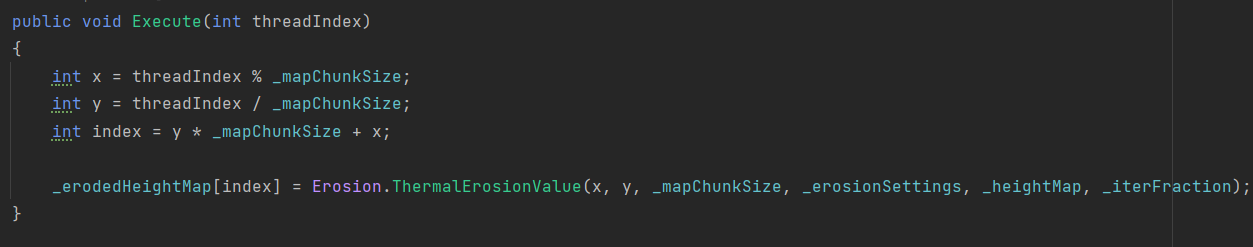
\includegraphics[width=1\textwidth]{img/codes/ExecuteErosionJob.png}
\caption{Implementación del método Execute de ErosionJob.}
\end{figure}

La erosión es un componente esencial para simular procesos realistas de degradación del terreno, como el suavizado de pendientes y la reducción de la aspereza. Su aplicación repetida a lo largo de varios ciclos permite modelar la evolución del terreno con el tiempo.
\subsubsection{Generación de Texturas del Terreno}

La generación de texturas del terreno se encarga de convertir el mapa de colores (colorMap) obtenido durante la generación de alturas en una textura adecuada para su visualización en el terreno. Esto se logra utilizando la clase \texttt{TextureGenerator}.

\subsubsection{Generación de texturas}

\begin{enumerate}
    \item \texttt{TextureFromColourMap}: Este método toma un arreglo de colores (\texttt{colourMap}), junto con el ancho y alto deseados, y crea una textura 2D a partir de estos datos. Configura la textura con un modo de filtrado (\texttt{Point}) y un modo de envoltura de textura que normaliza los valores. Luego, asigna los colores del \texttt{colourMap} y aplica la textura.

    \begin{figure}[h]
    \centering
    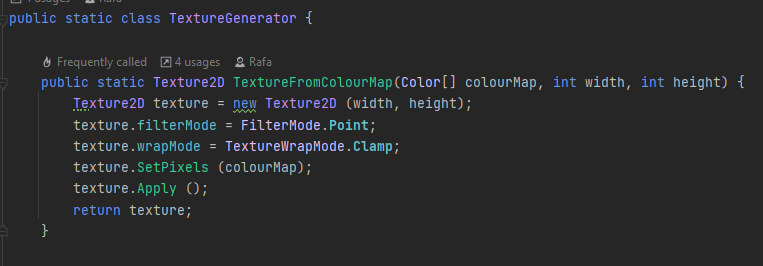
\includegraphics[width=0.85\textwidth]{img/codes/TextureColor.png}
    \caption{Implementación del método de generación de texturas.}
    \end{figure}
    \newpage
    \item \texttt{Uso en la Clase TerrainChunk}:En la clase \texttt{TerrainChunk}, específicamente en el método \texttt{OnMapDataReceived}, se utiliza la clase \texttt{TextureGenerator} para crear una textura a partir del mapa de colores (\texttt{colourMap}) contenido en el objeto \texttt{MapData} recibido. Luego, esta textura se asigna al material del terreno para su visualización en el objeto \texttt{\_meshRenderer}. A continuación se muestra el fragmento relevante de código:
    \begin{figure}[h]
        \centering
        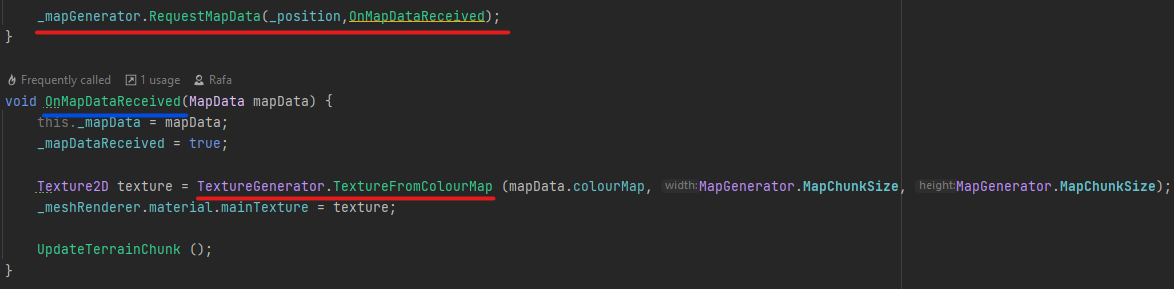
\includegraphics[width=0.85\textwidth]{img/codes/TexturizacionDeChunk.png}
        \caption{generación de textura al crearse un nuevo chunk.}
    \end{figure}
    
\end{enumerate}

\subsection{Elección de Estructuras de Datos y Tipos}

En esta sección se explicará por qué se han utilizado las estructuras de datos empleadas para la implementación de los trabajos y qué sentido tienen, dado que la elección de las estructuras viene en buena parte marcada por necesidades de implementación y optimización del rendimiento.

\subsubsection{Uso de structs en Jobs:}
El sistema de trabajos de Unity requiere que los trabajos sean tipos "no administrados", por lo que no pueden contener referencias a objetos. Las clases en C\# pueden contener referencias a otros objetos, lo que las hace más complejas y difíciles de optimizar. Esto se debe a que Job System está diseñado para funcionar con Burst Compiler, un compilador que optimiza el código generando código de máquina altamente optimizado que puede ejecutarse más rápido que el código C\# normal. Burst Compiler funciona mejor con tipos de datos simples que se pueden optimizar fácilmente, como las structs, por lo tanto, el uso de clases en el Job System de Unity puede provocar problemas de rendimiento, y es por esto que es preferible usar structs en lugar de clases, razón por la cual se han utilizado para el proyecto.

\subsubsection{NativeArrays:} 
El uso de NativeArrays en lugar de arrays de C\# se debe a que Burst Compiler está preparado para trabajar con estructuras de datos que permiten una optimización del código al pasarlo a lenguaje máquina. Los NativeArrays, a diferencia de los arrays normales, tienen una gestión de memoria eficiente, con posiciones contiguas donde almacenar los datos, de manera que no se produce fragmentación como sí podría ocurrir en los arrays de C\#. También almacenan los datos en zonas diferentes de la memoria que facilitan el acceso de manera más rápida y contribuyen a la eficiencia. Además, están preparados para que haya un acceso concurrente seguro de varios hilos a los datos que almacenan, por lo que permiten un manejo transparente al desarrollador de la concurrencia.

\subsubsection{Elección del tipo de Job:}
El tipo de job que se ha utilizado para el procesamiento de los vértices es IJobParallelFor, el cual divide el procesamiento de un número de posiciones de un array que se le pasa como parámetro en el método Schedule entre varios hilos, de manera óptima al ser un tipo de dato predefinido para ello. Dado que el tratamiento de los mapas de alturas y la creación de la malla es iterativo en su versión secuencial, el tener que paralelizar los bucles es una tarea que se realiza de manera óptima al usar un IJobParallelFor.


% Esta parte del código toma los datos de color del terreno, los convierte en una textura y luego asigna esa textura al material del terreno, lo que permite visualizar el terreno de manera adecuada en la escena de Unity.

% \subsection{Resolución de Problemas}

% En esta subsección, se abordan los problemas encontrados durante el desarrollo del sistema y se describe cómo se resolvieron. Se incluyen soluciones a desafíos específicos relacionados con la generación de terreno procedural en Unity.

% \begin{enumerate}
%     \item \textbf{Continuidad entre los chunks:}
%     \item \textbf{Separación entre los chunks:}
%     \item \textbf{Depresión de las zonas con agua:}
%     \item \textbf{Problemas de optimización temporal:}
%     \item \textbf{Problemas de optimización de memoria:}
%     \item \textbf{Problemas con continuidad de bordes al erosionar:}
%     \item \textbf{Problemas con rendimiento al erosionar:}
%     \item \textbf{Problemas con parametrización coherente:}
% \end{enumerate}